\documentclass[../main.tex]{subfiles}
\begin{document}

\section{Sinn}

\subsection{Ziel der Implementierung}

Die Entwicklung des hier beschriebenen Schreibassistenten verfolgt das Ziel, ein innovatives \glslink{glos:ki}{KI}-Werkzeug zu entwickeln, welches vor allem Schüler und Studenten bei dem Verfassen 
unterschiedlicher Texte unterstützt. Die von Studenten häufig genutzten Text-Editoren wie beispielsweise Overleaf sollen nicht ersetzt werden. Stattdessen soll eine Möglichkeit geboten werden, 
\glslink{glos:ki}{KI}-Chats mit unterschiedlichen \glslink{glos:llm}{LLM}s übersichtlich zu sammeln. Es soll wie in \autoref{sec:nachteile} beschrieben eine Art "`Augmented Intelligence"' geschaffen werden, welche die Effizienz während des Schreibprozesses 
steigert, jedoch nicht das Verfassen des gesamten Textes übernimmt. Im Gegensatz zu den in \autoref{sec:bereitsBestehendeLoesungen} beschriebenen bereits bestehenden Lösungen, sollen die verschiedenen \glslink{glos:ki}{KI}-Chats 
übersichtlich und spezifisch zu Textabschnitten angelegt werden können. Zu einem Textabschnitt sollen mehrere \glslink{glos:ki}{KI}-Chats mit unterschiedlichen Modellen erstellt und abgespeichert 
werden können. Durch das Sammeln der \glslink{glos:ki}{KI}-Gespräche soll ein übersichtlicheres Arbeiten ermöglicht werden. Zudem kann der Nutzer die von der \glslink{glos:ki}{KI} erhaltenen Antworten kommentieren, um 
sich Gedanken zu möglichen Verbesserungen oder der Relevanz der generierten Antwort für den entstehenden Text zu merken.\\
Das Nutzerinterface des Schreibassistenten soll intuitiv und verständlich gestaltet sein. Dazu wird ein schlichtes Design verwendet. Um auch unerfahrenen Nutzern den Umgang mit 
generativer \glslink{glos:ki}{KI} zu vereinfachen, werden die in \autoref{ch:anforderungen} identifizierten Anforderungen an ein \glslink{glos:ki}{KI}-Werkzeug umgesetzt. Dies beinhaltet Tooltips an Knöpfen, welche mit der 
\glslink{glos:ki}{KI}-Funktionalität verbunden sind. Diese sollen die Funktionalität für den Nutzer verständlich erklären. Jeder Nutzer soll so nachvollziehen können, welchen Einfluss eine Eingabe in 
einem bestimmten Textfeld oder eine Auswahl aus einem Drop-Down Menü auf die generierte Antwort haben. Zudem wird der Nutzer bei dem Anlegen eines neuen Projektes gewarnt, dass 
\glslink{glos:ki}{KI}-Modell halluzinieren können. Damit soll, ähnlich wie in der in \autoref{ch:anforderungen} behandelten Studie, die Akzeptanz von \glslink{glos:ki}{KI}-generierten Misinformationen verringert werden. Dadurch 
soll das Risiko, dass Fehlinformationen in die Arbeiten der Schüler und Studenten gelangen, verringert werden. Die Nutzer sollen angeregt werden, die von der \glslink{glos:ki}{KI} generierten Inhalte 
kritisch zu hinterfragen.\\
Auch bei der Formulierung von Prompts sollen die Nutzer unterstützt werden. Da bereits die kleinste Änderung im Prompt oder in der Reihenfolge der mitgegebenen Informationen großen 
Einfluss auf die \glslink{glos:ki}{KI}-Antwort haben kann, sind verlässliche und reproduzierbare Arbeitsabläufe schwer zu erreichen\cite{creativeWriting}. Dies soll durch das Zusammensetzen vorgefertigter 
Prompts im Backend umgangen werden. Zudem soll so die Nutzung auch für \glslink{glos:ki}{KI}-Unerfahrene erleichtert werden. Dazu werden Prompts für folgende in \autoref{sec:vorteile} identifizierten 
Einsatzmöglichkeiten bereitgestellt: umformulieren, zusammenfassen, Text aus Stichpunkten formulieren, Synonyme finden, Grammatik und Rechtschreibung prüfen und Feedback geben. Zudem soll das KI-Modell
Schülern Sachverhältnisse erklären können, um das Textverständnis zu fördern. 


\subsection{Anwendungsfälle}

Der Schreibassistent wird für unterschiedliche Anwendungsfälle entwickelt: \\
Zum einen soll dem Nutzer ein Werkzeug geboten werden, mit welchem er strukturiert verschiedene \glslink{glos:ki}{KI}-Modelle nutzen kann. Die bereitgestellten vorgefertigten Prompts sollen die 
Effizienz während des Schreibprozesses weiter steigern. Darüber hinaus sind jedoch auch nutzerdefinierte Prompts möglich. Das generierte \glslink{glos:ki}{KI}-Nutzungsverzeichnis kann an als eine Art 
Quellenverzeichnis an wissenschaftliche Arbeiten angehangen werden. Abgebildet wird dort das verwendete \glslink{glos:ki}{KI}-Modell, die Aufgabe welche das Modell 
übernehmen sollte beziehungsweise der Prompt, welchen der Nutzer eingegeben hat, sowie das Datum, an welchem die Anfrage gestellt wurde. In diesem KI-Nutzungsverzeichnis werden nur 
Prompts zu den gespeicherten Chats angeführt. Dadurch wird vermieden, dass Chats vermerkt werden, deren Ergebnisse nicht in die Arbeit eingeflossen sind, und entstehende Verzeichnis 
bleibt übersichtlicher.\\ 
Der zweite Anwendungsfall ist der sogenannte Schülermodus. Durch das Einschränken der Funktionalität soll ein Werkzeug zur Verfügung gestellt werden, welches auch zu 
Unterrichtszwecken verwendet werden kann. So sollen Schüler den Umgang mit generativer \glslink{glos:ki}{KI} erlernen, ohne dabei den gesamten Text von dem \glslink{glos:ki}{KI}-Modell schreiben zu lassen. Die 
entstandenen Texte sind immer noch die Eigenleistung des Schülers, jedoch kann durch den Einsatz des Schreibassistenten der Schreibprozess effizienter gestaltet werden, was die in 
\autoref{sec:vorteile} beschriebenen Vorteile mit sich bringt. Der Schüler kann aus den bereits vorgefertigten Aufgaben für die \glslink{glos:ki}{KI} wählen, jedoch keinen eigenen Prompt verwenden. Dadurch soll 
verhindert werden, dass gesamte Texte \glslink{glos:ki}{KI}-generiert werden. Zudem wird anders als im normalen Modus jeder Chat im \glslink{glos:ki}{KI}-Nutzungsverzeichnis vermerkt. Dies sorgt für bessere 
Nachvollziehbarkeit der \glslink{glos:ki}{KI}-Nutzung für Lehrkräfte.\\ 
Zuletzt soll der Schreibassistent auch beim Schreiben von benoteten Arbeiten während des Unterrichts eingesetzt werden können. Dazu dient der Prüfungsmodus. Es kann eine bestimmte 
Zeit eingestellt werden, in welcher der Schüler seinen Text bearbeiten kann. Ist diese Zeit abgelaufen, wird der entstandene Text automatisch abgegeben. Das \glslink{glos:ki}{KI}-Nutzungsverzeichnis 
wird wie im Schülermodus erstellt, sodass alle \glslink{glos:ki}{KI}-Chats später erkennbar sind. Zudem wird das Öffnen anderer Projekte oder Tabs verhindert. Sollte ein Schüler versuchen, über ein 
anderes Projekt im Schreibassistenten oder über eine andere Anwendung \glslink{glos:ki}{KI} oder andere Hilfsmittel zu verwenden, wird die Arbeit automatisch abgegeben. Dadurch soll sichergestellt 
werden, dass das Schreiben der Arbeit weiterhin eine eigene Leistung des Schülers ist. Die \glslink{glos:ki}{KI} hilft bei der Formulierung und mit der Rechtschreibung des Textes, den Inhalt selbst 
muss jedoch der Schüler verfassen. Insgesamt soll eine sichere Umgebung zur Verfügung gestellt werden, wodurch der Einsatz generativer \glslink{glos:ki}{KI} auch während des Unterrichts ermöglicht wird.


\section{Verwendete Technologien}

Das Frontend des Schreibassistenten ist mithilfe des Frameworks React erstellt worden. Diese JavaScript Bibliothek verfolgt einen komponentenbasierten Ansatz. Da jedes Element als 
eigene Komponente behandelt wird, erhöht sich die Wiederverwendbarkeit des Codes. Alle benutzerdefinierten Komponenten werden direkt oder indirekt der von React bereitgestellten 
App-Komponente untergeordnet. So entsteht eine Baumstruktur mit der App-Komponente als Startknoten. (Alex Banks, 2020; Hutsulyak, 2024; Ks, 2022)\\
React TSX wurde für die Entwicklung des Schreibassistenten vor allem aufgrund seiner Performanz und Dynamik gewählt. React TypeScript bringt den Vorteil der Typisierung mit sich, 
wodurch der geschriebene Code weniger fehleranfällig ist.\cite{react1,react2} \\
Zur Umsetzung des Designs wird Cascading Style Cheats (CSS) verwendet. Diese Sprache bietet ebenfalls den Vorteil der Wiederverwendbarkeit durch das erstellen eigener CSS-Klassen. 
Im Gegensatz zur Verwendung von CSS-Frameworks ermöglicht die Nutzung von reinem CSS eine größere Flexibilität. \\ 
Das Backend ist mit dem Web-Framework FastAPI erstellt worden. Dieses Python-Framework zeichnet sich vor allem durch gute Performanz aus. Die bereitgestellte Typisierung sowie die 
Verwendung von Datenmodellen sorgen für eine verbesserte Code-Qualität\cite{fastapi}.\\ Python als verwendete Programmiersprache sorgt ebenfalls für eine erhöhte Effizienz. Die Einfachheit dieser 
Programmiersprache sowie die weite Verbreitung erleichtern den Entwicklungsprozess. Zudem gibt es viele zusätzliche Bibliotheken für Python.\cite{python}\\
Eine dieser Bibliotheken, welche auch für die Implementierung des Schreibassistenten genutzt wurde, ist SQLAlchemy. Diese bietet eine objektorientierte Abstraktionsschicht für den 
Zugriff auf die Datenbank. Somit kann mit Python-Klassen statt mit reinen SQL-Abfragen gearbeitet werden. Zudem können komplexe Abfragen und Bedingungen mit Python-Code formuliert 
werden. Somit wird der Code übersichtlicher und einfacher zu warten. Der Zugriff auf die verwendete SQLite Datenbank wird damit vereinfacht, jedoch wäre auch ein späterer Umstieg auf 
eine andere Datenbank mit wenig Aufwand möglich, falls eine leistungsfähigere Datenbank benötigt werden sollte.\cite{SQLAlchemy}\\
Für die Einbindung der \glslink{glos:ki}{KI}-Modelle wurde Ollama verwendet. Ollama ist eine Open-Source-Software, welche die Ausführung von \glslink{glos:llm}{LLM}s lokal auf dem Rechner ermöglicht. Ollama stellt eine 
API zur Verfügung, durch die diese Funktionalitäten eingebunden werden können. So können verschiedene Modelle genutzt werden. Ollama übernimmt während der Nutzung den Wechsel 
zwischen den Modellen. Dies verhindert, dass zwei Modelle gleichzeitig Rechenressourcen beanspruchen und erhöht somit die Performanz.\cite{ollamaSchreibassi,ollamaTechnologie}

\section{Verwendete \glslink{glos:ki}{KI}-Modelle}
\label{sec:kiModelle}

Mit Ollama können verschiedene \glslink{glos:ki}{KI}-Modelle während des Schreibprozesses verwendet werden. Alle diese Modell laufen lokal auf dem Rechner des Nutzers, wodurch mögliche Datenschutzprobleme, 
wie in \autoref{sec:datenschutz} beschrieben, umgangen werden. So kann der implementierte Schreibassistent beispielsweise auch im Rahmen eines duales Studiums zum Verfassen von 
Praxisphasenberichten ohne datenschutzrechtliche Bedenken des Partnerunternehmens verwendet werden.\\ 
Der Nutzer soll frei zwischen mehreren \glslink{glos:ki}{KI}-Modellen wählen können. Durch die Verwendung von Ollama ist es dem Nutzer auch möglich, selber zu entscheiden, welche Modelle zur Verfügung 
stehen sollen. Um jedoch unerfahrenen Nutzern die Arbeit mit dem \glslink{glos:ki}{KI}-Werkzeug zu vereinfachen, soll zu jeder Aufgabe mit bereits vorgefertigtem Prompt ein bestimmtes KI-Modell 
vorgeschlagen werden, welches diese Aufgabe wahrscheinlich am erfolgreichsten löst.\\ 
Dazu wurden einige Modelle miteinander verglichen. Diese wurden aufgrund der Spezialisierung auf die deutsche Sprache und wegen ihrer Größe ausgewählt. Modelle mit einer 
Parameteranzahl zwischen acht und zwölf Milliarden bieten qualitative Antworten und laufen dennoch auf neueren Laptops relativ performant. Aufgrund des zeitlichen Rahmens dieses 
Studienprojektes wurden die Modelle nicht einzeln gebenchmarkt, sondern lediglich stichprobenartig für jeden Aufgabentyp getestet und die gegebenen Antworten anschließend auf 
Ausdruck, grammatikalische Korrektheit und Inhalt überprüft. Dabei ergaben sich folgende Ergebnisse: 

\begin{itemize}

\item \textbf{lukasmalkmus/llama3-sauerkraut} ist ein acht Milliarden Parameter großes Llama-3 Modell mit Feinabstimmung auf die deutsche Sprache\cite{sauerkraut}. Im Test antwortet das Modell stellenweise auf Englisch, obwohl im Prompt eine deutsche Antwort gefordert wird. Einige deutsche Begriffe aus dem Prompt gehen verloren oder werden durch ähnlich klingende englische Begriffe ersetzt. Das Modell wird im Schreibassistenten für keine Aufgabe verwendet.

\item \textbf{mayflowergmbh/wiedervereinigung} ist die Kombination aus mehreren auf Mistral basierenden \glslink{glos:ki}{KI}-Modellen mit einer Größe von sieben Milliarden Parametern und ebenfalls auf die deutsche Sprache abgestimmt\cite{wiedervereinigung}. Im Test fügt es häufig neuen Inhalt hinzu, statt sich auf die eigentlich geforderte Aufgabe zu begrenzen. Das Modell wird im Schreibassistenten für keine Aufgabe verwendet.

\item \textbf{mayflowergmbh/wiederchat} ist eine sieben Milliarden Parameter große erweiterte Variante des Wiedervereinigungs-Modells führt während des Tests Prompts meist nicht vollständig aus\cite{wiederchat}. Für das Zusammenfassen von Texten gibt es jedoch die beste Antwort, da lediglich Inhalt aus dem Text widergegeben wurde und das Format den geforderten Stichpunkten entsprach. Dieses Modell wird im Schreibassistenten für das Zusammenfassen von Texten vorgeschlagen.

\item \textbf{jobautomation/OpenEuroLLM-German} ist eine für deutschsprachige Antworten optimierte Version von Gemma 3, welche trainiert wurde, grammatikalisch korrekte Antworten ohne fremdsprachige Fachwörter zu geben\cite{openeurollm}. Während des Tests antwortet es vollständig, gut strukturiert und meist dem gegebenen Prompt entsprechend. Es wird für die Aufgabe, einen Text aus Stichpunkten zu formulieren, als Standard-Modell verwendet, da der entstehende Text gut formuliert und besser strukturiert war als der anderer Modelle. Ebenfalls wird es zum umformulieren des Textes vorgeschlagen, da der gegebene Text lediglich neu formuliert und nicht ergänzt wurde.  

\item \textbf{Gemma3} ist ein von Google entwickeltes Open Source \glslink{glos:ki}{KI}-Modell, welches aufgrund seiner Architektur auch auf Laptops performant läuft, und mit zwölf Milliarden Parametern das größte getestete Modell\cite{gemma3}. Da dieses Modell nicht auf die deutsche Sprache spezialisiert wurde, sind die Texte meist nicht gut formuliert. Als allgemeines Modell zum Finden von Synonymen und Geben von Feedback ist es jedoch sehr gut geeignet und wird daher für diese Aufgaben vorgeschlagen. 

\end{itemize}

[vllt noch was dazu sagen, wie man sich neue modelle ziehen kann]

\section{Aufbau der Datenbank}
\begin{figure}[h!]
  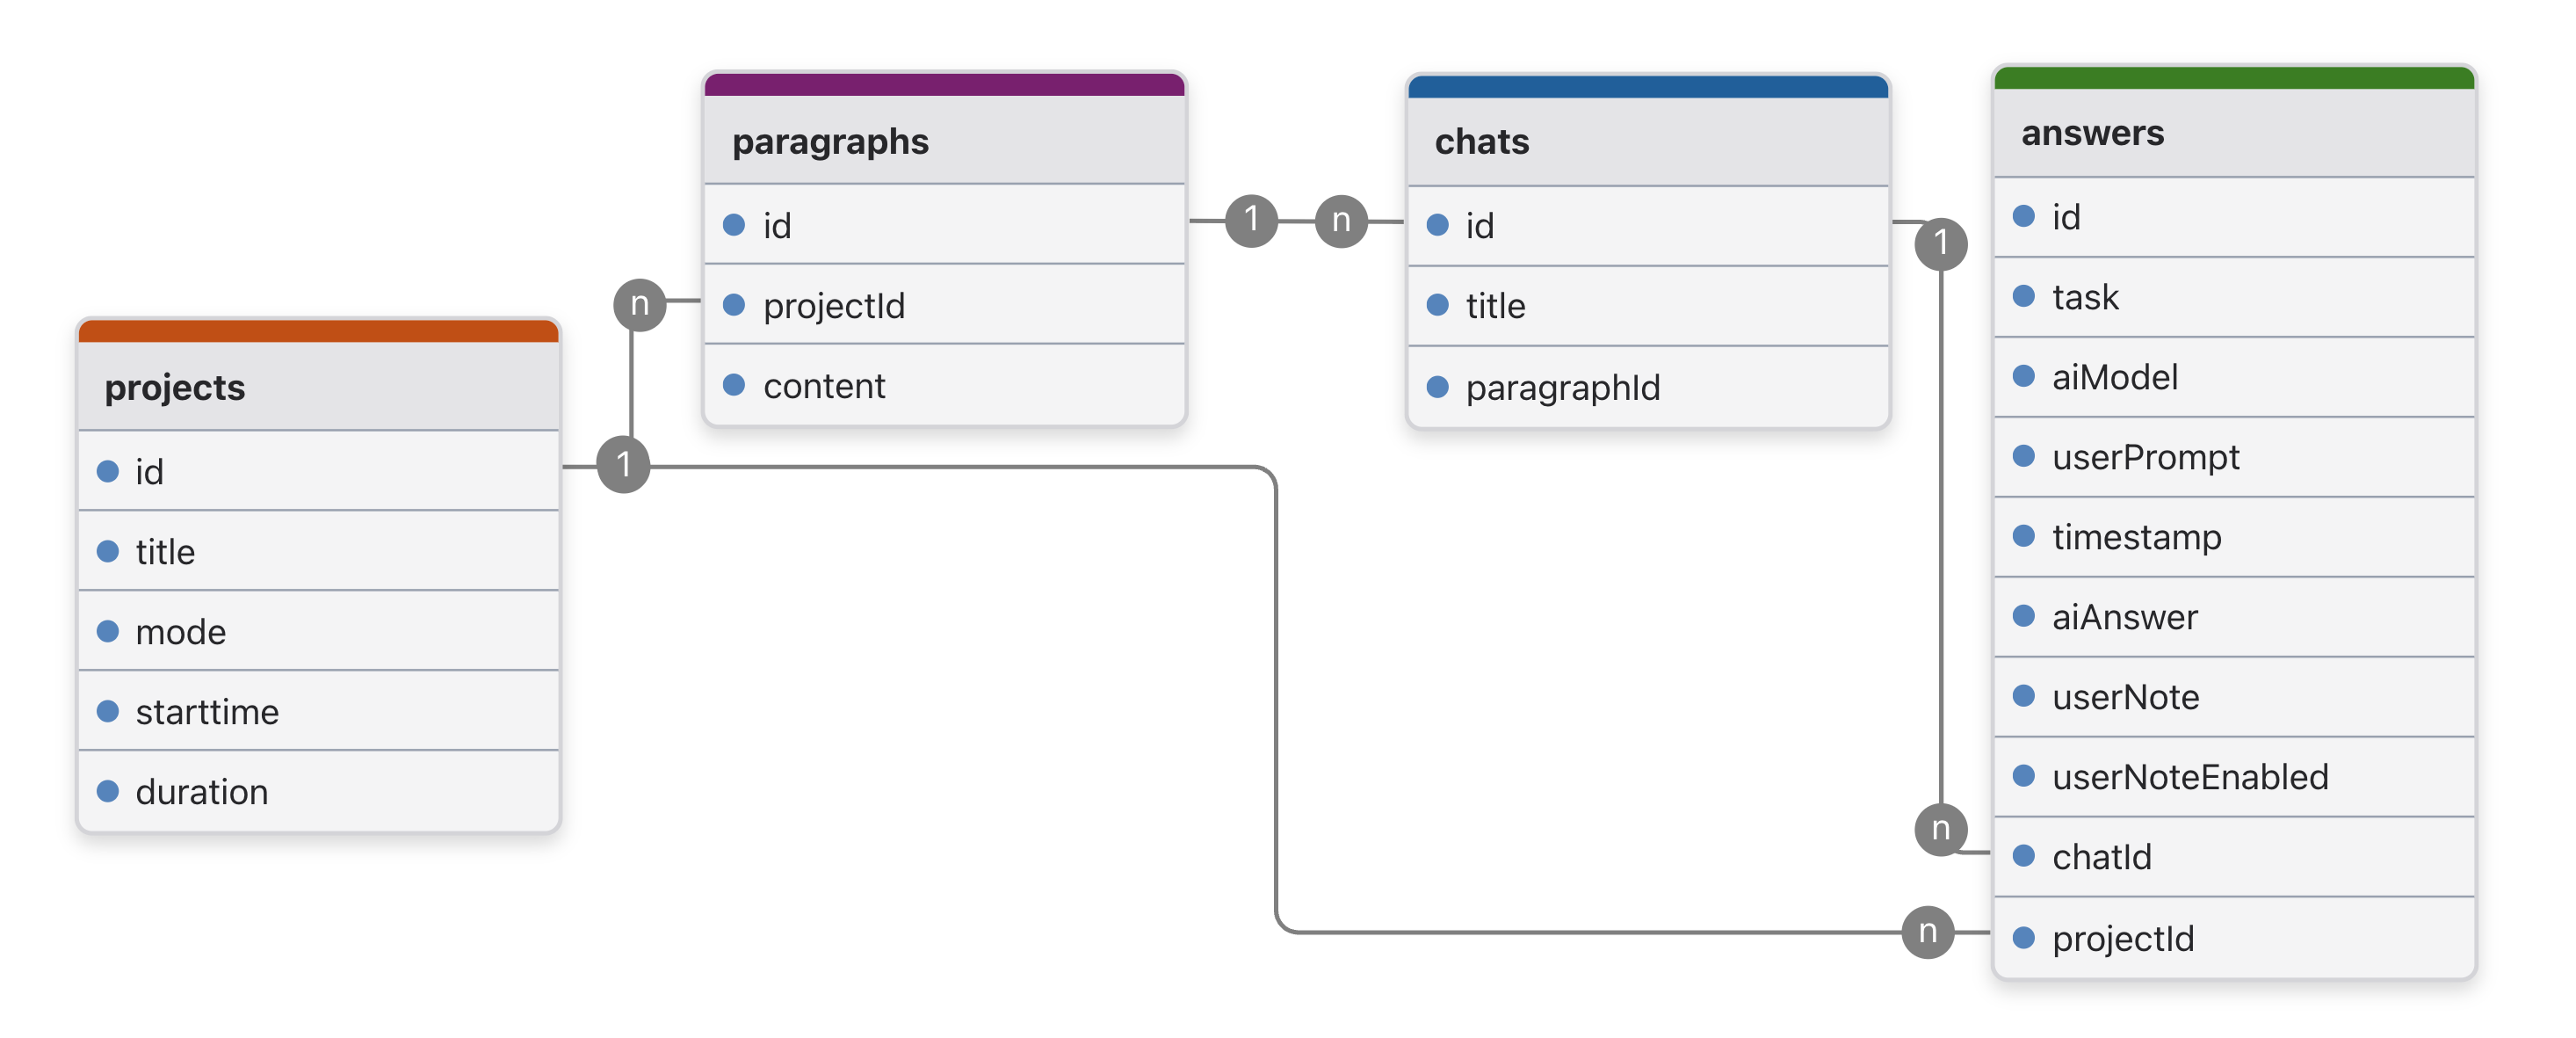
\includegraphics[scale=0.14]{bilder/Datenbank.png}
  \caption{Datenbankschema}
  \label{fig:data}
\end{figure}
Die Datenbank wird in Abb \ref{fig:data} schematisch dargestellt. Die Datenbank hat insgesamt vier miteinander verknüpfte Tabellen. Die erste Tabelle speichert alle zu einem Projekt gehörenden 
Informationen. Neben der ID und dem Projekttitel hat diese Tabelle noch das Feld "`mode"', welches den Modus des Projektes angibt. Modus 0 steht dabei für den normalen Modus ohne 
Einschränkungen. Modus 1 und 2 haben die Einschränkungen des Schülermodus, wobei in Modus 2 der Text nur in einer bestimmten Zeit bearbeitet werden kann. Um im Frontend einen Timer 
zu ermöglichen, werden im Backend die Startzeit sowie die Dauer des Timers vermerkt. Schließlich gibt es noch den Modus 3, welcher der Abgegeben-Modus ist. In diesem kann das Projekt 
nicht weiter bearbeitet, sondern nur gelesen und das \glslink{glos:ki}{KI}-Nutzungsverzeichnis generiert werden.\\
Jedes Projekt kann mehrere Paragraphen haben. Diese sind der vom Nutzer geschriebene Text. Jedem Paragraphen können wiederum mehrere \glslink{glos:ki}{KI}-Chats zugeordnet werden. Die Chats haben 
jeweils einen Titel und können mehrere "`Answers"' beinhalten. Die "`Answers"' stellen die eigentliche Konversation mit der \glslink{glos:ki}{KI} dar. Sie bestehen aus der Anfrage des Nutzers mit allen 
Informationen die gespeichert werden sollen, sowie einem optionalen Kommentar, welcher aktiviert sein kann. Ist der Kommentar aktiviert, so wird er der \glslink{glos:ki}{KI} bei den nächsten Anfragen 
im Chat mitgegeben, sonst nicht. Außerdem hat jede Answer einen Zeitstempel, welcher für das \glslink{glos:ki}{KI}-Nutzungsverzeichnis relevant ist.\\
Zusätzlich zu den beschriebenen Verknüpfungen der Tabellen gibt es noch eine Verknüpfung zwischen den Projekten und den Answers. Diese sorgt dafür, dass im Schülermodus, in welchem 
alle \glslink{glos:ki}{KI}-Anfragen gespeichert werden sollen, selbst beim Löschen des Paragraphen die Anfrage nicht verloren geht. So können im \glslink{glos:ki}{KI}-Nutzungsverzeichnis die \glslink{glos:ki}{KI}-Anfragen für gelöschte 
Paragraphen gespeichert werden, was die Nachvollziehbarkeit für den benotenden Lehrer erhöht.



\section{Frontend und Backend}
\begin{figure}[h!]
  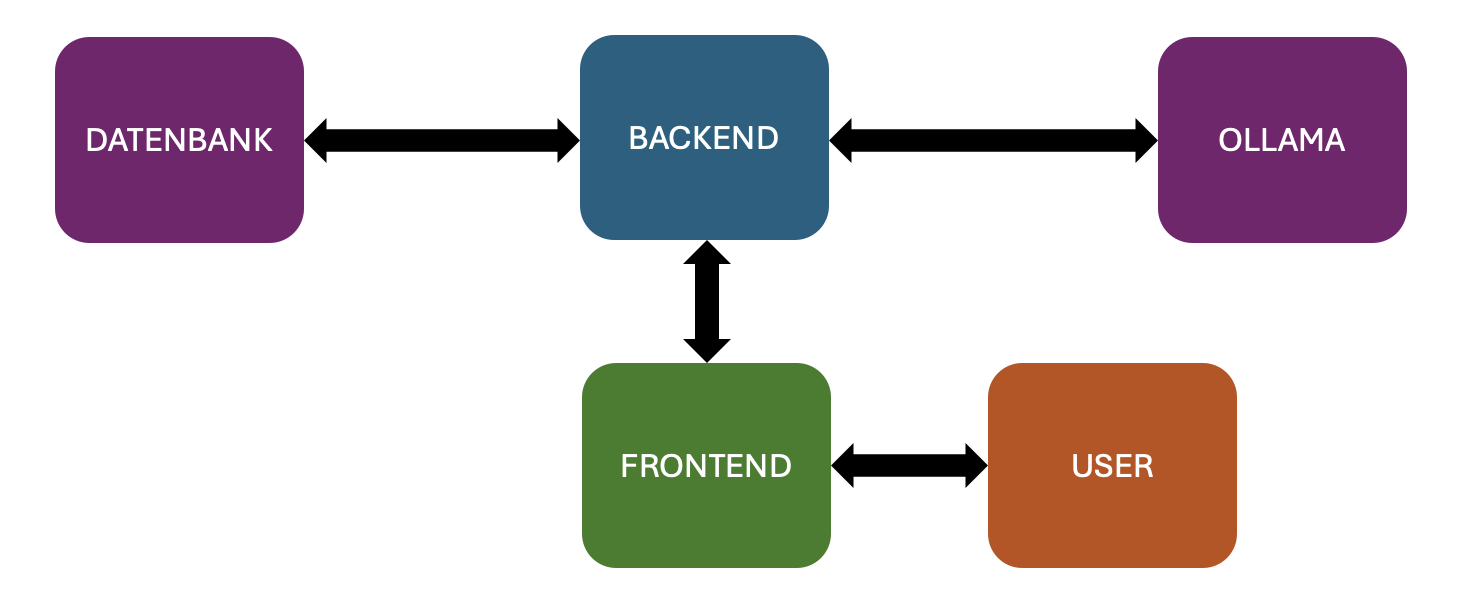
\includegraphics[scale=0.6]{bilder/Architektur.png}
  \caption{Architekturschema}
  \label{fig:architecture}
\end{figure}
Das Backend stellt die nötigen Endpunkte für das Frontend zur Verfügung, um Projekte, Paragraphen, Chats und Answers zu erstellen, zu löschen und abzurufen, oder bereits gespeicherte 
Informationen zu ändern, sowie Aufrufe an Ollama zu senden (Abb \ref{fig:architecture}). Das Frontend nutzt diese Endpunkte, um die Funktionalität dem Nutzer bereitzustellen.\\

Beim Erstellen eines Projektes in Modus 2 kann eine Zeit festgelegt werden, in welcher der Text bearbeitet werden kann. Die verbleibende Zeit wird über einen Timer angezeigt. Ist 
dieser abgelaufen, wird der Modus automatisch auf Modus 3 gesetzt, sowie das \glslink{glos:ki}{KI}-Nutzungsverzeichnis und die Text-PDF generiert und heruntergeladen. Um zu verhindern, dass Schüler 
während der Arbeit andere Tabs oder Anwendungen auf ihrem Gerät öffnen, wird auch beim Verlassen des Browsertabs die Arbeit automatisch abgegeben. Dies wird über das sogenannte 
"`blur-event"' erreicht, welches ausgelöst wird, wenn das entsprechende Element den Fokus verliert\cite{react-onblur}. Auch beim Schließen der entsprechenden Projektansicht-Seite durch das Zurückkehren 
auf den Startbildschirm wird das Projekt abgegeben, um zu verhindern, dass Schüler über ein nicht funktionsmäßig eingeschränktes Projekt andere KI-Anfragen stellen. Schließlich kann 
das Projekt noch durch das Klicken auf den "`Abgeben"'-Knopf abgegeben werden.\\
Beim Generieren des \glslink{glos:ki}{KI}-Nutzungsverzeichnisses für ein Projekt wird zuerst eine Anfrage an das Backend gestellt, welche ein JSON-formatiertes Objekt aller 
notwendigen Informationen zurückgibt. Dieses wird im Frontend als PDF formatiert und kann heruntergeladen werden.

\section{KI-Funktionalität}

Die \glslink{glos:ki}{KI}-Modelle werden, wie in \autoref{sec:kiModelle} beschrieben, mithilfe von Ollama eingebunden. Um einen \glslink{glos:ki}{KI}-Aufruf zu tätigen, wird eine Anfrage vom Backend an die lokale 
Ollama-API geschickt. Dafür benötigt Ollama die Information, welches \glslink{glos:ki}{KI}-Modell verwendet werden soll, und welcher Inhalt mitgegeben werden soll. Dabei wird zwischen dem User-Prompt 
und dem System-Prompt unterschieden. Insgesamt müssen aus dem Backend also drei verschiedene Variablen mitgegeben werden. Dazu werden folgende Angaben zusammengefasst: Die Aufgabe, 
der bisherige Chatverlauf, der Inhalt des Paragraphen, eventuell die Nutzerkommentare zu den \glslink{glos:ki}{KI}-Antworten, sowie weitere im Frontend bestimmte Felder. Bevor diese Informationen dem 
\glslink{glos:ki}{KI}-Modell geschickt werden, müssen sie zusammengesetzt werden. Dabei wird für jede der vorgegebenen Aufgaben ein Prompt angefügt, welcher der \glslink{glos:ki}{KI} 
mitteilt, was für eine Art Inhalt generiert werden soll. Diese Prompts wurden manuell getestet. Die Antwort des \glslink{glos:ki}{KI}-Modells wurde bewertet und der Prompt entsprechend angepasst, bis der generierte Inhalt zufriedenstellend war.
Außerdem wird für jede Aufgabe ein empfohlenes \glslink{glos:llm}{LLM} gewählt, welches die Aufgabe am besten erfüllt. Die Prompts sind auf Deutsch,da der Schreibassistent auf deutsche 
Sprache spezialisiert ist. Zudem lieferten englische Prompts während der Tests keine signifikant anderen Ergebnisse. 

\section{Problema}

Während der Entwicklung und Implementierung der Funktionalität traten mehrere Probleme auf.\\
Eine Herausforderung bestand darin, dass der Schreibassistent auch problemlos funktionieren soll, wenn Schüler während des Schreibens keine \glslink{glos:ki}{KI}-Chats erstellen. In diesem Fall würde 
bei dem Generieren des \glslink{glos:ki}{KI}-Nutzungsverzeichnisses ein Fehler geworfen werden, da keine zu dem Projekt gehörenden Answers gefunden werden können. Dieses Backend-Fehler wird nun 
abgefangen. Stattdessen wird  das \glslink{glos:ki}{KI}-Nutzungsverzeichnis mit dem Schriftzug "`keine \glslink{glos:ki}{KI} verwendet"' generiert.\\
Ein weiteres Problem bestand darin, dass Variablen im Frontend nur temporär gespeichert werden und bei den erneuten Laden der Seite verloren gehen. Das führte zum Zurücksetzen des 
Timers. Um dies zu umgehen werden im Backend die Werte "`Starttime"' und "`Duration"', also der Startzeitpunkt des Timers und die Dauer der Bearbeitungszeit, gespeichert.\\ 
Schließlich besteht bei der Nutzung des Schreibassistenten noch die Gefahr des sogenannten Prompt-Injectings, also dass Schüler im Falle von eingeschränkter Funktionalität versuchen 
könnten, diese Einschränkungen zu umgehen, indem sie im Paragraphen oder in bestimmten Eingabefeldern ganze Prompts eingeben. Dies soll so gut es geht verhindert werden.\\ 
Dafür gibt es verschiedene Möglichkeiten: Eine Option ist, die Eingabe direkt zu filtern, um vorher zu überprüfen, ob ein Prompt-Injection-Versuch stattfindet. Dies könnte zum Beispiel 
über ein zwischengeschaltetes \glslink{glos:llm}{LLM} geschehen, welches darauf trainiert wurde, Prompt-Injection zu erkennen. Des Weiteren könnten bestimmte Wörter oder Phrasen statisch verboten werden. 
Es wurde sich gegen diese Optionen entschieden, da das zwischengeschaltete \glslink{glos:ki}{KI}-Modell die Performanz einschränken würde. Das Verbieten einzelner Phrasen könnte während des 
Schreibprozesses sehr einschränkend wirken.\cite{promptinjection}\\
Eine andere Möglichkeit wäre das Filtern der Ausgabe. Da sich die Ausgabe eines umformulierten Textes jedoch kaum von der eines neu generierten unterscheidet, ist dies auch keine 
zureichende Lösung. Schließlich wurde eine Kombination aus Parametrisierung und Prompt-Engineering umgesetzt. Bei den meisten Eingabefeldern werden die Möglichkeiten auf wenige 
festgelegte Optionen reduziert, sodass dort keine Eingabe von benutzerdefinierten Texten möglich ist. Bei einigen Feldern lässt sich dies jedoch nicht vermeiden. In diesem Fall wurde 
Prompt-Engineering angewendet, um der \glslink{glos:ki}{KI} möglichst genau aufzuzeigen, welche Teile des Prompts vom Nutzer kommen und was die eigentliche Aufgabe ist.\\

\end{document}